\section{Implementation}

\subsection{Hardware}
Diagrammet viser interaktioner mellem systemets hardware dele. Dette er vist med et \textit{internal block diagram (IBD)}. Diagrammer beskriver kommunikationen mellem hardware blokkene. Her specificeres hvad der kommunikeres mellem blokkene og hvilke interfaces det foregår via. \\
\begin{figure}[H]
	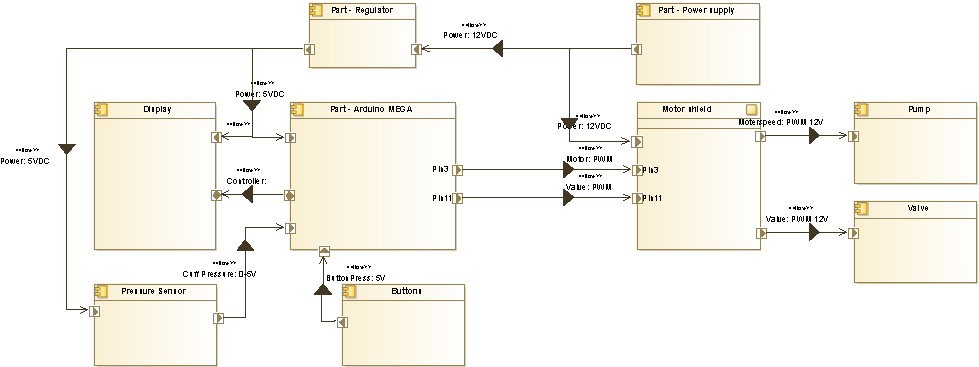
\includegraphics[width=\textwidth]{SystemArkitektur/pdfs/IBD-Hardware-crop}
	\caption{Internal block diagram over flow for hardwaren i \textit{Konditioneringsapparatet}}
\end{figure}

\subsubsection{Beskrivelse af hardware}
Se beskrivelser i kapitel \ref{title:systemPart}

\subsubsection{Arduino Mega 2560 og Motor Shield}
Til udvikling af prototypen bruges en Arduino Mega med en AtMega2560 processor og et 12V motor shield. Se oversigt tegning på figur \ref{fig:arduinoMega}. \\
\begin{figure}[H]
	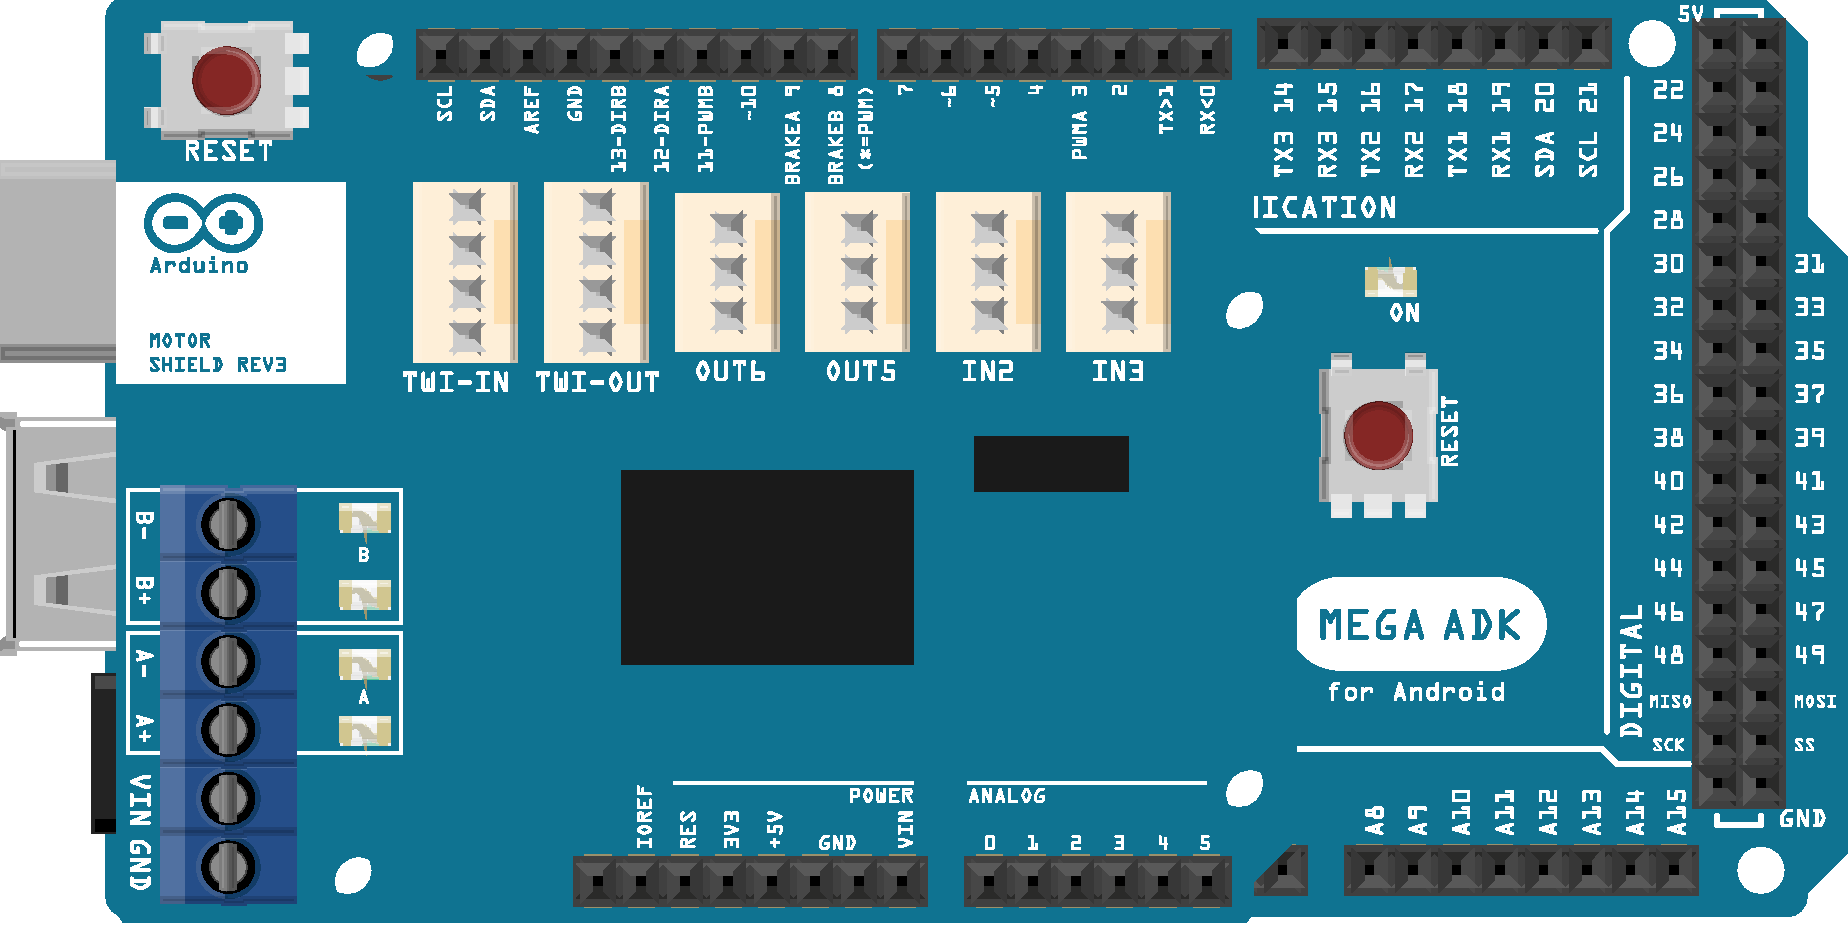
\includegraphics[width=\textwidth]{SystemArkitektur/pdfs/MegaPlusShield-crop.pdf}
	\caption{Arduino Mega med 12V motor shield monteret} \label{fig:arduinoMega}
\end{figure}


\subsection{Software}
\textit{Konditioneringsapparet} består kun af ét software system og det kræver ikke flere software systemer for at apparatet fungere. Dette giver derfor et simpelt struktur for softwaren 

\subsubsection{Klasse diagram}
Diagrammet præsentere software klasser med funktioner og de er opdelt i hver sit namespace. Denne struktur er valgt for at opnå høj samhørighed og lav kobling.
\begin{figure}[H]
	\centering
	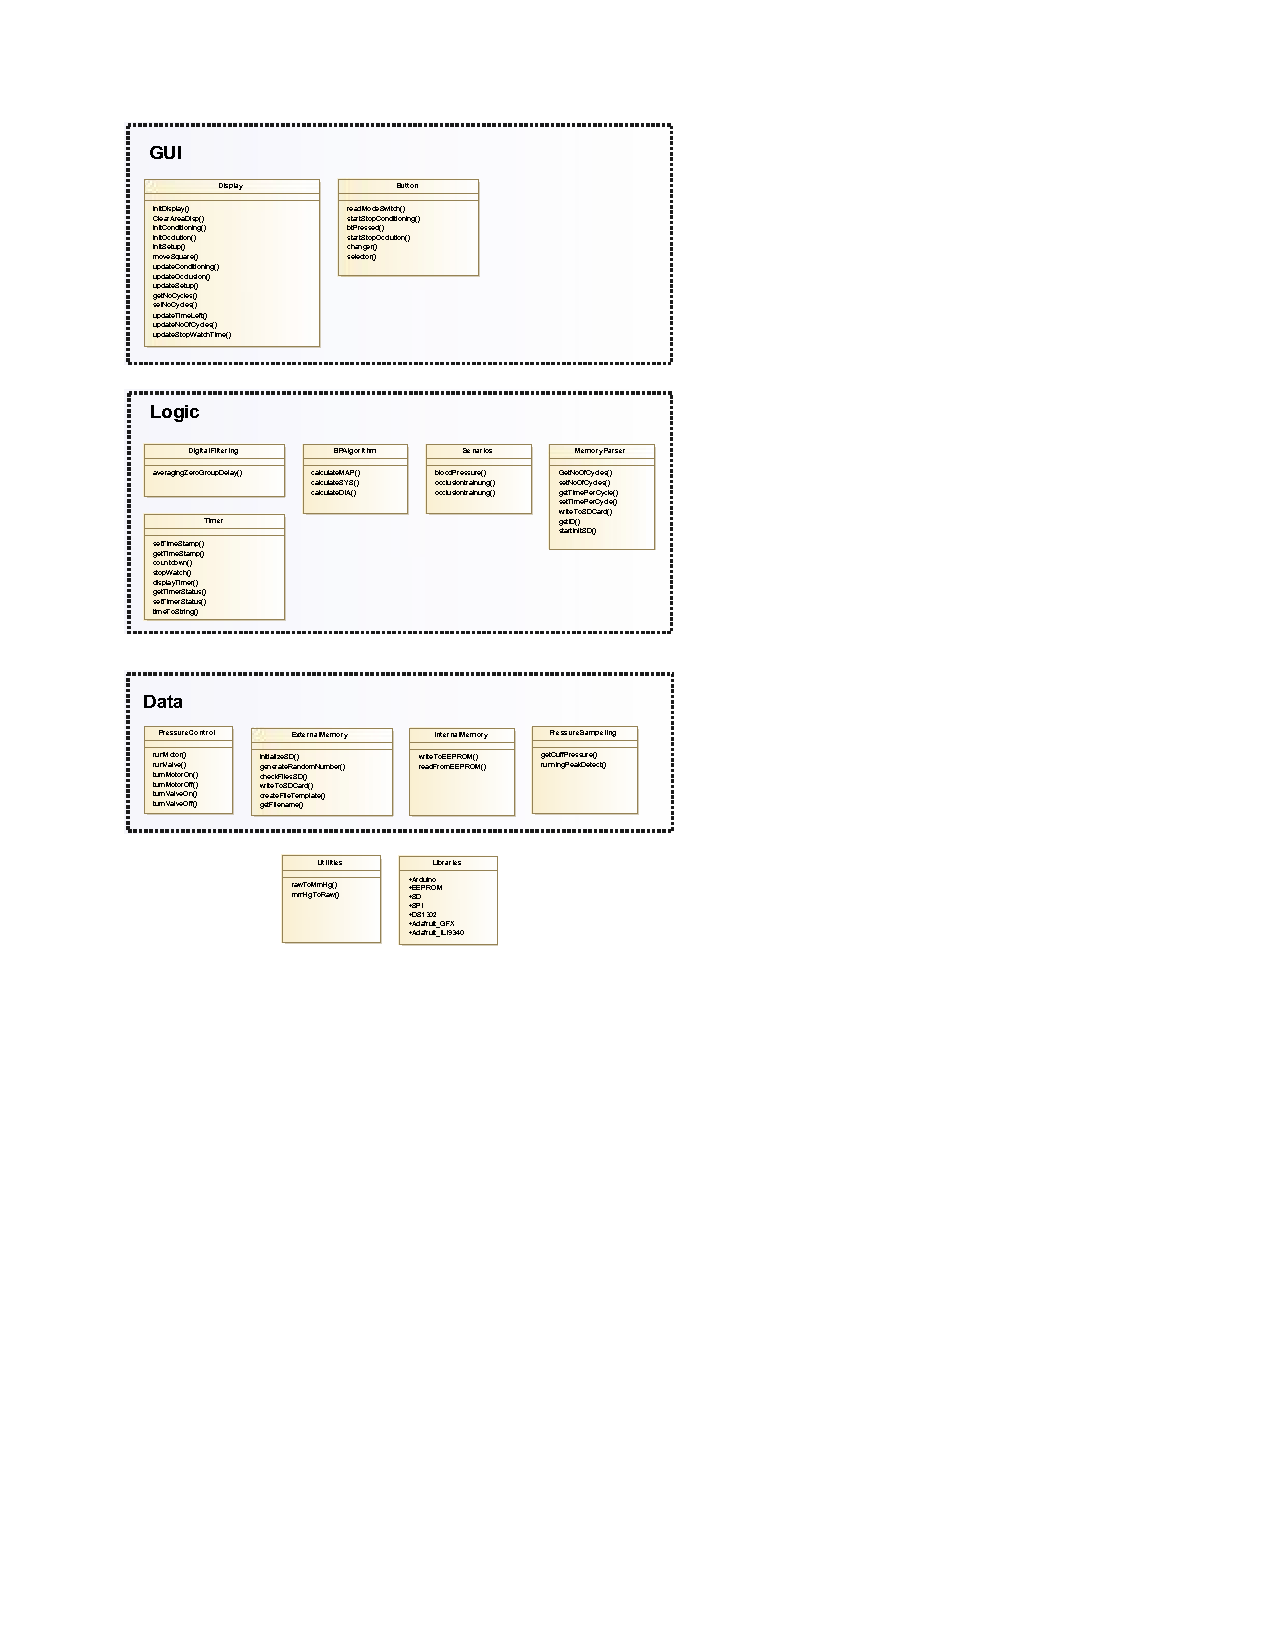
\includegraphics[width=0.8\textwidth]{SystemArkitektur/pdfs/ClassDiagram.pdf}
	\caption{Class diagram for softwaren i \textit{Konditioneringsapparatet}}
\end{figure}


\subsubsection{Sprog}
\begin{itemize}
	\item \textbf{C++} - brugt til at skrive source code til arduino
	\item \textbf{SysML} - brugt til udvikling af system diagrammer
\end{itemize}

\subsubsection{3-lags modellen}
Softwaren er struktureret efter 3-lags princippet. Dette design er valgt for at give klare grænseflader og ansvarsfordeling. De tre lags er præsentationslaget, logik laget og datalaget. Lagdelingen giver stor fleksibilitet fordi det er nemmere at vedligeholde og genbruge kode fra et bestemt lag uden at den influere med andre lag. De tre lag er repræsenteret som hvert sit namespace i software arkitekturen

\subsubsection{Udviklingsværktøjer}

\textbf{Eclipse} \\
IDE til udvikling af C og C++. Dette miljø bruges til at skrive koden til arduinoen og dermed styringen af prototypen. Der er valgt versionen: “Juno Service Release”. Denne version understøtter integration af Arduino’ eget IDE, samtidig med at man kan gøre brug af Eclipses programmerings funktioner.  

\textbf{Arduino IDE} \\
Arduinos eget udviklingsmiljø bruges som et plugin via Eclipse. Den brugte version er 1.5.5. Grundet manglende funktion er det blevet fravalgt at bruge Arduino IDE alene. 

\textbf{Git, GitHub Desktop og SmartGit} \\
Til versionsstyring af til projekt dokumentation og source code. Bachelor gruppen har købt et privat repository grundede den igangværende patentsag. Som bruger interface for git er blevet brugt henholdsvis GitHub Desktop og SmartGit

\textbf{Eksterne biblioteker} \\
Arduino biblioteker 
\begin{itemize}
\item EEPROM - muliggøre operationer på arduinoen indbyggede hukommelse
\item SD - muliggøre operationer med SD kort
\item TFT - funktioner til at bruge tft displays til arduino 
\end{itemize}

